\vspace{30px}\section{NTC thermistors}
In contrast to the PTC thermistor, there is the negative-temperature-coefficient thermistor. This device reduces its resistivity when the temperature rises.

\todo{Make NTC introduction a little longer}





\subsection{Chrateristics}
The NTC thermistor and the PTC thermistor, even though their functioning is opposite, have the same characteristic equation. As aforementioned, the equation that describes the behavior of the resistance $R$ in relationship with the ambient temperature $T$ is the following \cite{Chen20091103}:

\begin{equation*}
    R = R_0 \, e^{\, \beta\left( \frac{1}{T} - \frac{1}{T_0}\right)}
\end{equation*}

\noindent Where $R$ is the resistance at temperature $T$, which should be measured in Kelvin degrees, and $R_0$ is the resistance value measured at operating temperature $T_0$. The $\beta$ coefficient describes the thermister constant which varies on temperature and materials used to build the device. It can be calculated using the same formula described in the PTC thermistors:

\begin{equation*}
    \beta = \frac{\ln{\frac{R_2}{R_1}}}{\frac{1}{T_2} - \frac{1}{T_1}}
\end{equation*}

\noindent By assuming that when $T_1 = 298.15 K = 25^\circ C$, $R_1 = 10k\Omega$ and when $T_2 = 358.15 K = 85^\circ C$. $R_2 = 1.4k\Omega$, it is possible to plot the resistance-temperature relationship of a negative temperature coefficient thermistor. As shown in figure \ref{fig:NTC_logarithmic}, the curve shows that as the temperature rises, the resistance value decreases respecting the aforementioned equation.

\begin{figure}[h]
    \centering
    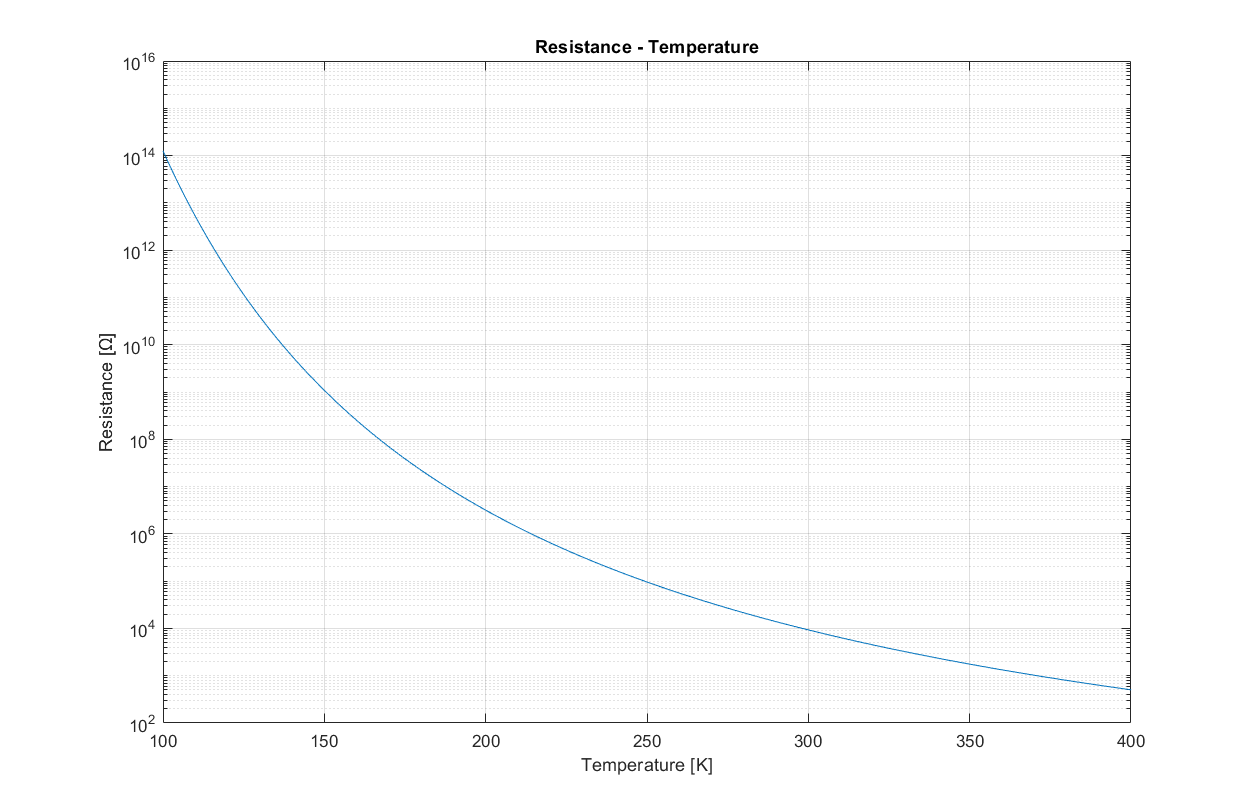
\includegraphics[width = .75\textwidth]{../res/plots/NTC_logarithmic.png}
    \label{fig:NTC_logarithmic}
    \caption{NTC resistance-temperature logarithmic curve, from -173°C to 326°C.}
\end{figure}

\FloatBarrier\noindent If the curve is restricted to more realistic temperature values (such as -13°C to 126°C), it's even more evident the inversely exponential curve which is described by the equation of the thermistor (figure \ref{fig:NTC_cartesian}).

\begin{figure}[h]
    \centering
    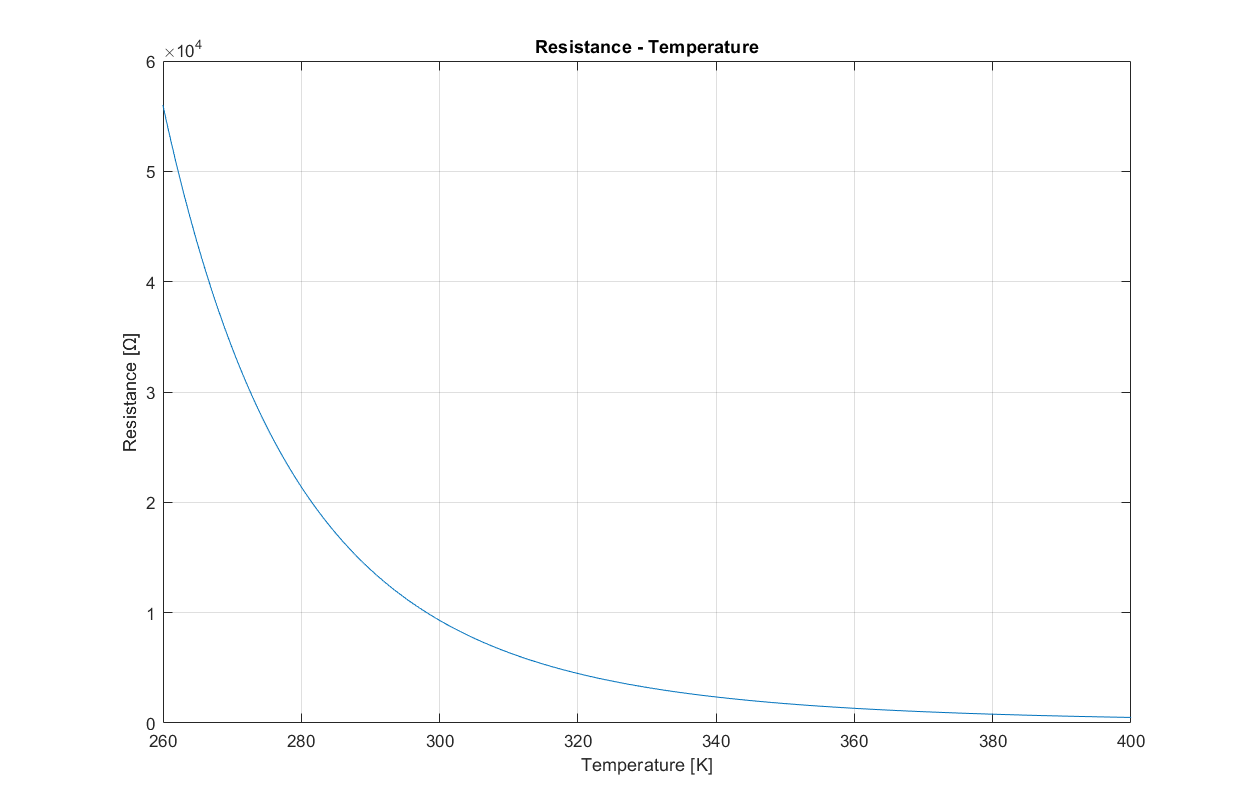
\includegraphics[width = .75\textwidth]{../res/plots/NTC_cartesian.png}
    \label{fig:NTC_cartesian}
    \caption{NTC resistance-temperature curve, limited between -13°C and 126°C.}
\end{figure}





\subsection{Applications}
As the posistor, also the NTC thermistor was used in space applications, specifically in the launch of the ETS-VI satellite and the H-II satellite \cite{Ishikawa1989116}.